\section{main.cpp File Reference}
\label{main_8cpp}\index{main.cpp@{main.cpp}}
{\tt \#include \char`\"{}main.h\char`\"{}}\par
{\tt \#include \char`\"{}mainwindow.h\char`\"{}}\par
{\tt \#include \char`\"{}appconfig.h\char`\"{}}\par
{\tt \#include \char`\"{}clipbrecords.h\char`\"{}}\par


Include dependency graph for main.cpp:\begin{figure}[H]
\begin{center}
\leavevmode
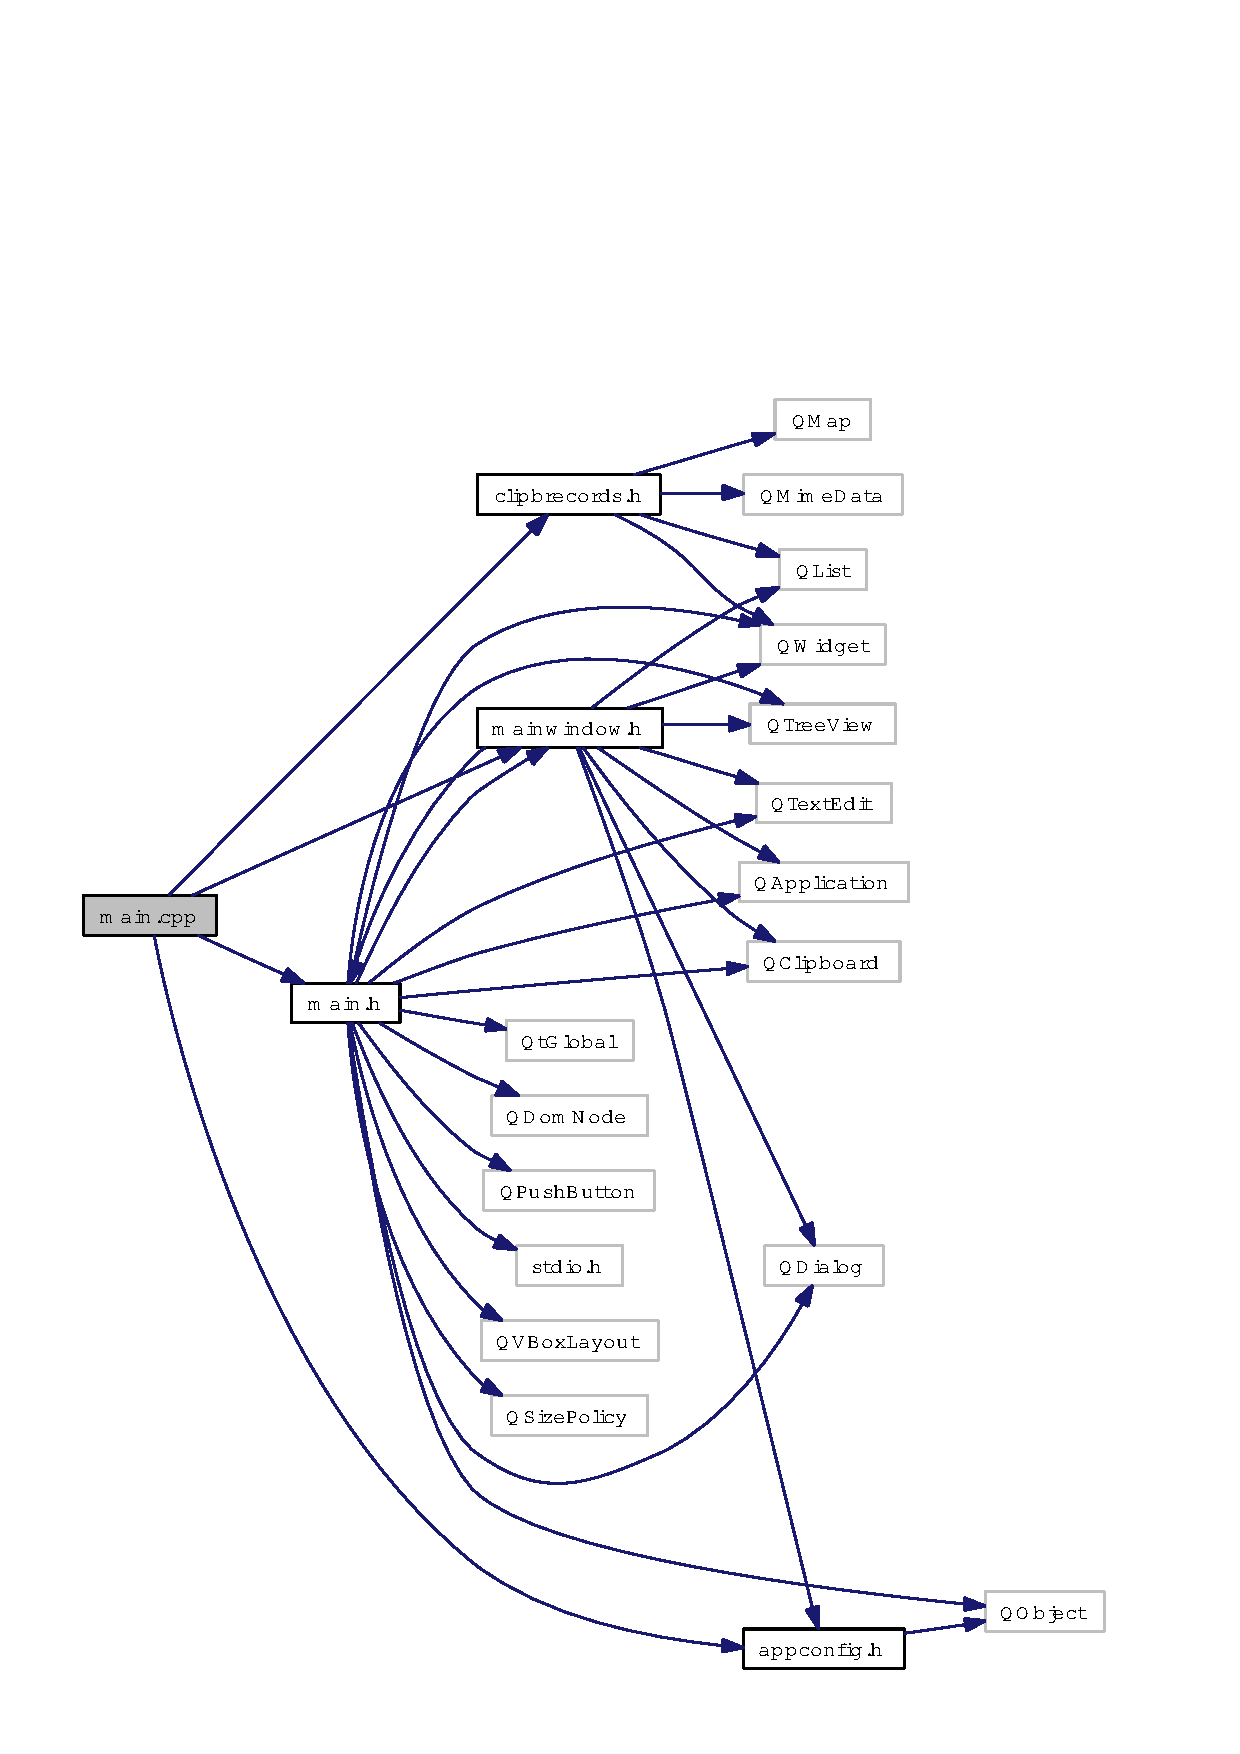
\includegraphics[width=267pt]{main_8cpp__incl}
\end{center}
\end{figure}
\subsection*{Functions}
\begin{CompactItemize}
\item 
void {\bf logprint} (char $\ast$lpsz\-Text,...)
\item 
void {\bf critical\_\-error} (QString message)
\item 
void {\bf info\_\-window} (QString i)
\item 
QString {\bf xmlnode\_\-to\_\-string} (QDom\-Node xmldata)
\item 
QString {\bf convert\_\-to\_\-lastnumformat} (int n)
\item 
void {\bf remove\_\-dir} (QString namedirfrom)
\item 
char $\ast$ {\bf from\-QString\-To\-Char} (const QString \&str)
\item 
void {\bf print\_\-object\_\-tree\_\-recurse} (QObject $\ast$pobj)
\item 
void {\bf print\_\-object\_\-tree} (void)
\item 
bool {\bf compare\_\-QString\-List\_\-len} (const QString\-List \&list1, const QString\-List \&list2)
\item 
int {\bf imax} (int x1, int x2)
\item 
int {\bf imin} (int x1, int x2)
\item 
int {\bf main} (int argc, char $\ast$$\ast$argv)
\end{CompactItemize}
\subsection*{Variables}
\begin{CompactItemize}
\item 
{\bf appconfig} {\bf mytetraconfig}
\item 
QObject $\ast$ {\bf mainwindowpointer}
\end{CompactItemize}


\subsection{Function Documentation}
\index{main.cpp@{main.cpp}!compare_QStringList_len@{compare\_\-QStringList\_\-len}}
\index{compare_QStringList_len@{compare\_\-QStringList\_\-len}!main.cpp@{main.cpp}}
\subsubsection{\setlength{\rightskip}{0pt plus 5cm}bool compare\_\-QString\-List\_\-len (const QString\-List \& {\em list1}, const QString\-List \& {\em list2})}\label{main_8cpp_4b9267e7db7804b40590ebb0aae4c257}




Definition at line 223 of file main.cpp.\index{main.cpp@{main.cpp}!convert_to_lastnumformat@{convert\_\-to\_\-lastnumformat}}
\index{convert_to_lastnumformat@{convert\_\-to\_\-lastnumformat}!main.cpp@{main.cpp}}
\subsubsection{\setlength{\rightskip}{0pt plus 5cm}QString convert\_\-to\_\-lastnumformat (int {\em n})}\label{main_8cpp_ec163ac31ec8c8183dc05762ecb4281d}




Definition at line 107 of file main.cpp.\index{main.cpp@{main.cpp}!critical_error@{critical\_\-error}}
\index{critical_error@{critical\_\-error}!main.cpp@{main.cpp}}
\subsubsection{\setlength{\rightskip}{0pt plus 5cm}void critical\_\-error (QString {\em message})}\label{main_8cpp_fe5e42a76086b3d9d2912f0c17ef0e59}




Definition at line 42 of file main.cpp.

Referenced by appconfig::appconfig(), Tree\-Item::data(), recordtabledata::get\_\-field(), infofieldenter::get\_\-field(), editrecord::get\_\-field(), recordtabledata::get\_\-fields(), appconfig::get\_\-parameter(), clipbrecords::get\_\-record(), recordtabledata::get\_\-text(), Tree\-Model::get\-Item(), recordtabledata::insert\_\-new\_\-record(), recordtablescreen::select(), appconfig::set\_\-addnewrecord\_\-expand\_\-info(), recordtabledata::set\_\-field(), metaeditor::set\_\-field(), infofieldenter::set\_\-field(), and editrecord::set\_\-field().

Here is the caller graph for this function:\begin{figure}[H]
\begin{center}
\leavevmode
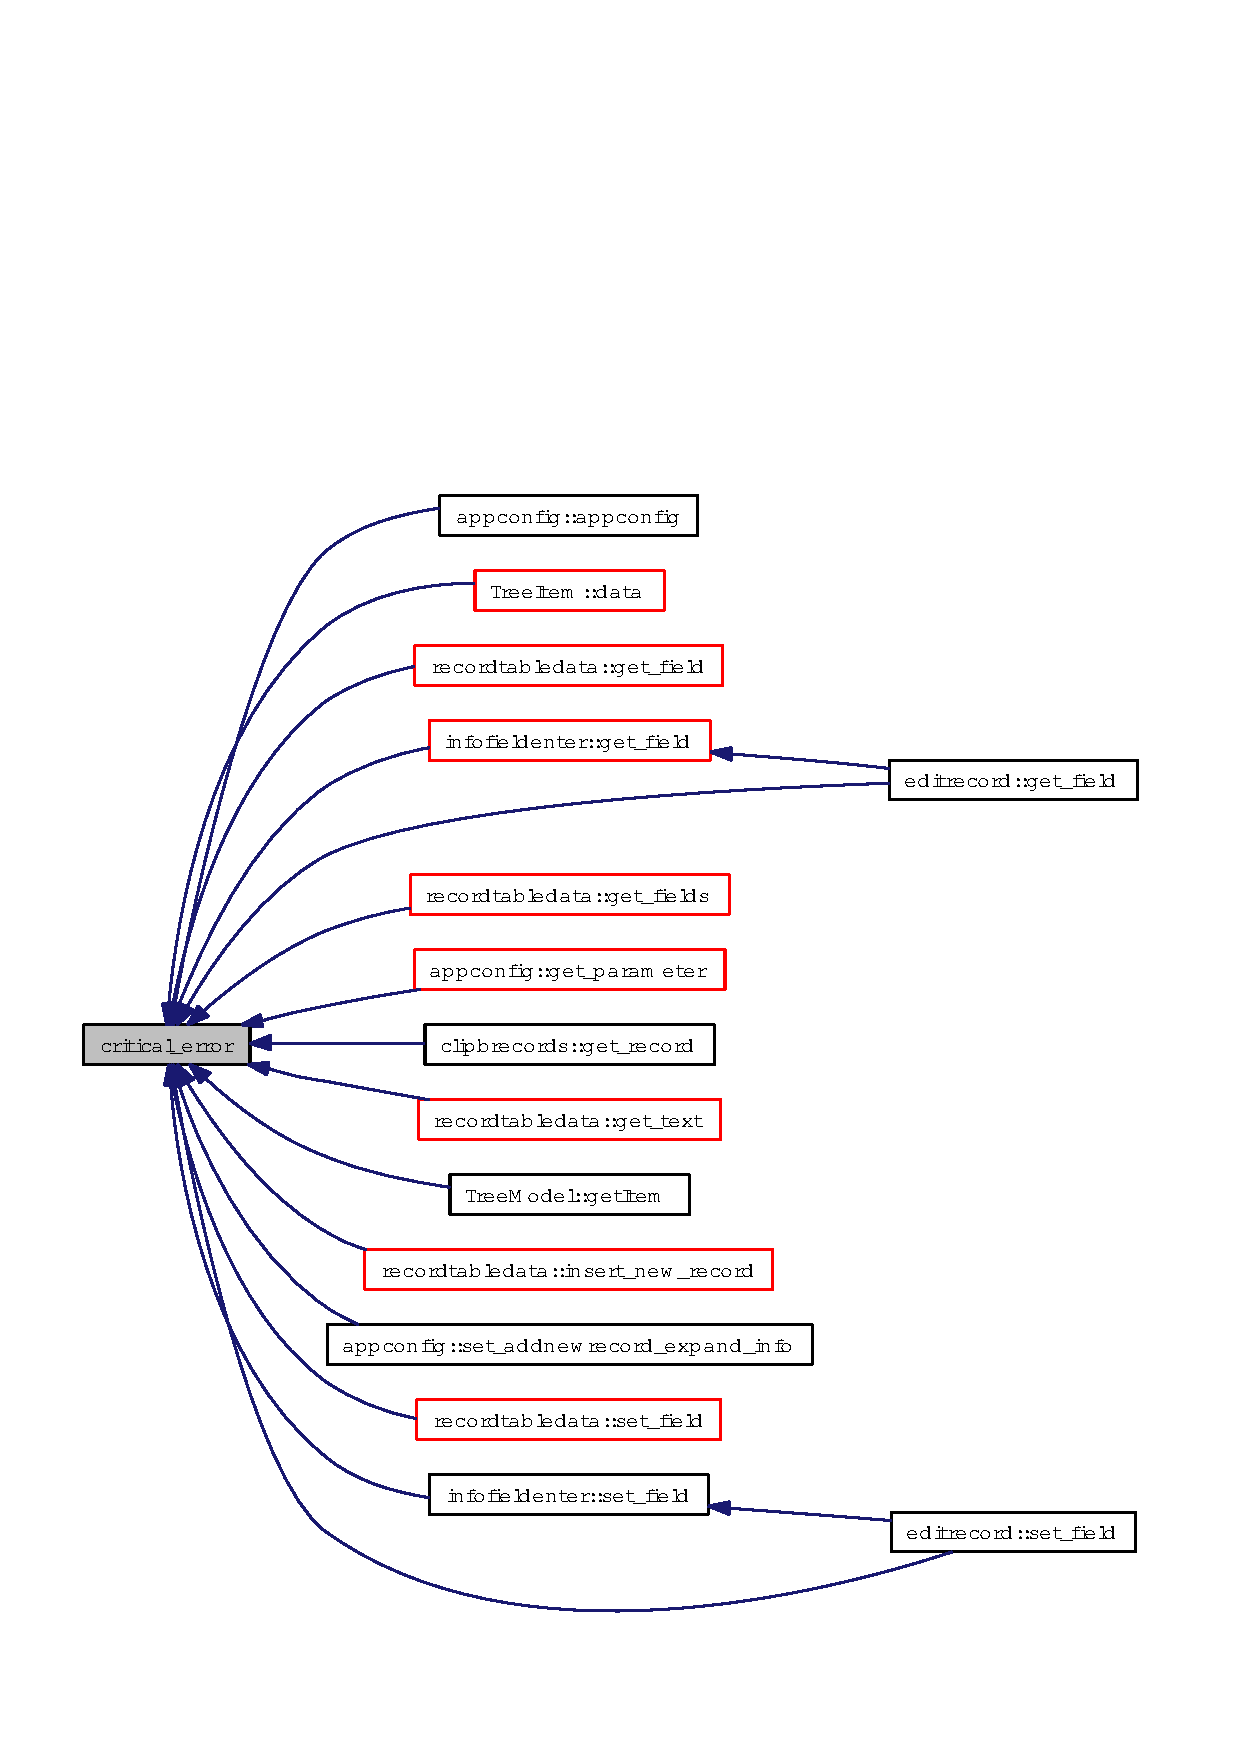
\includegraphics[width=275pt]{main_8cpp_fe5e42a76086b3d9d2912f0c17ef0e59_icgraph}
\end{center}
\end{figure}
\index{main.cpp@{main.cpp}!fromQStringToChar@{fromQStringToChar}}
\index{fromQStringToChar@{fromQStringToChar}!main.cpp@{main.cpp}}
\subsubsection{\setlength{\rightskip}{0pt plus 5cm}char$\ast$ from\-QString\-To\-Char (const QString \& {\em str})}\label{main_8cpp_0dda5f4014a4e3496449270026f6c149}




Definition at line 167 of file main.cpp.

Referenced by print\_\-object\_\-tree\_\-recurse().

Here is the caller graph for this function:\begin{figure}[H]
\begin{center}
\leavevmode
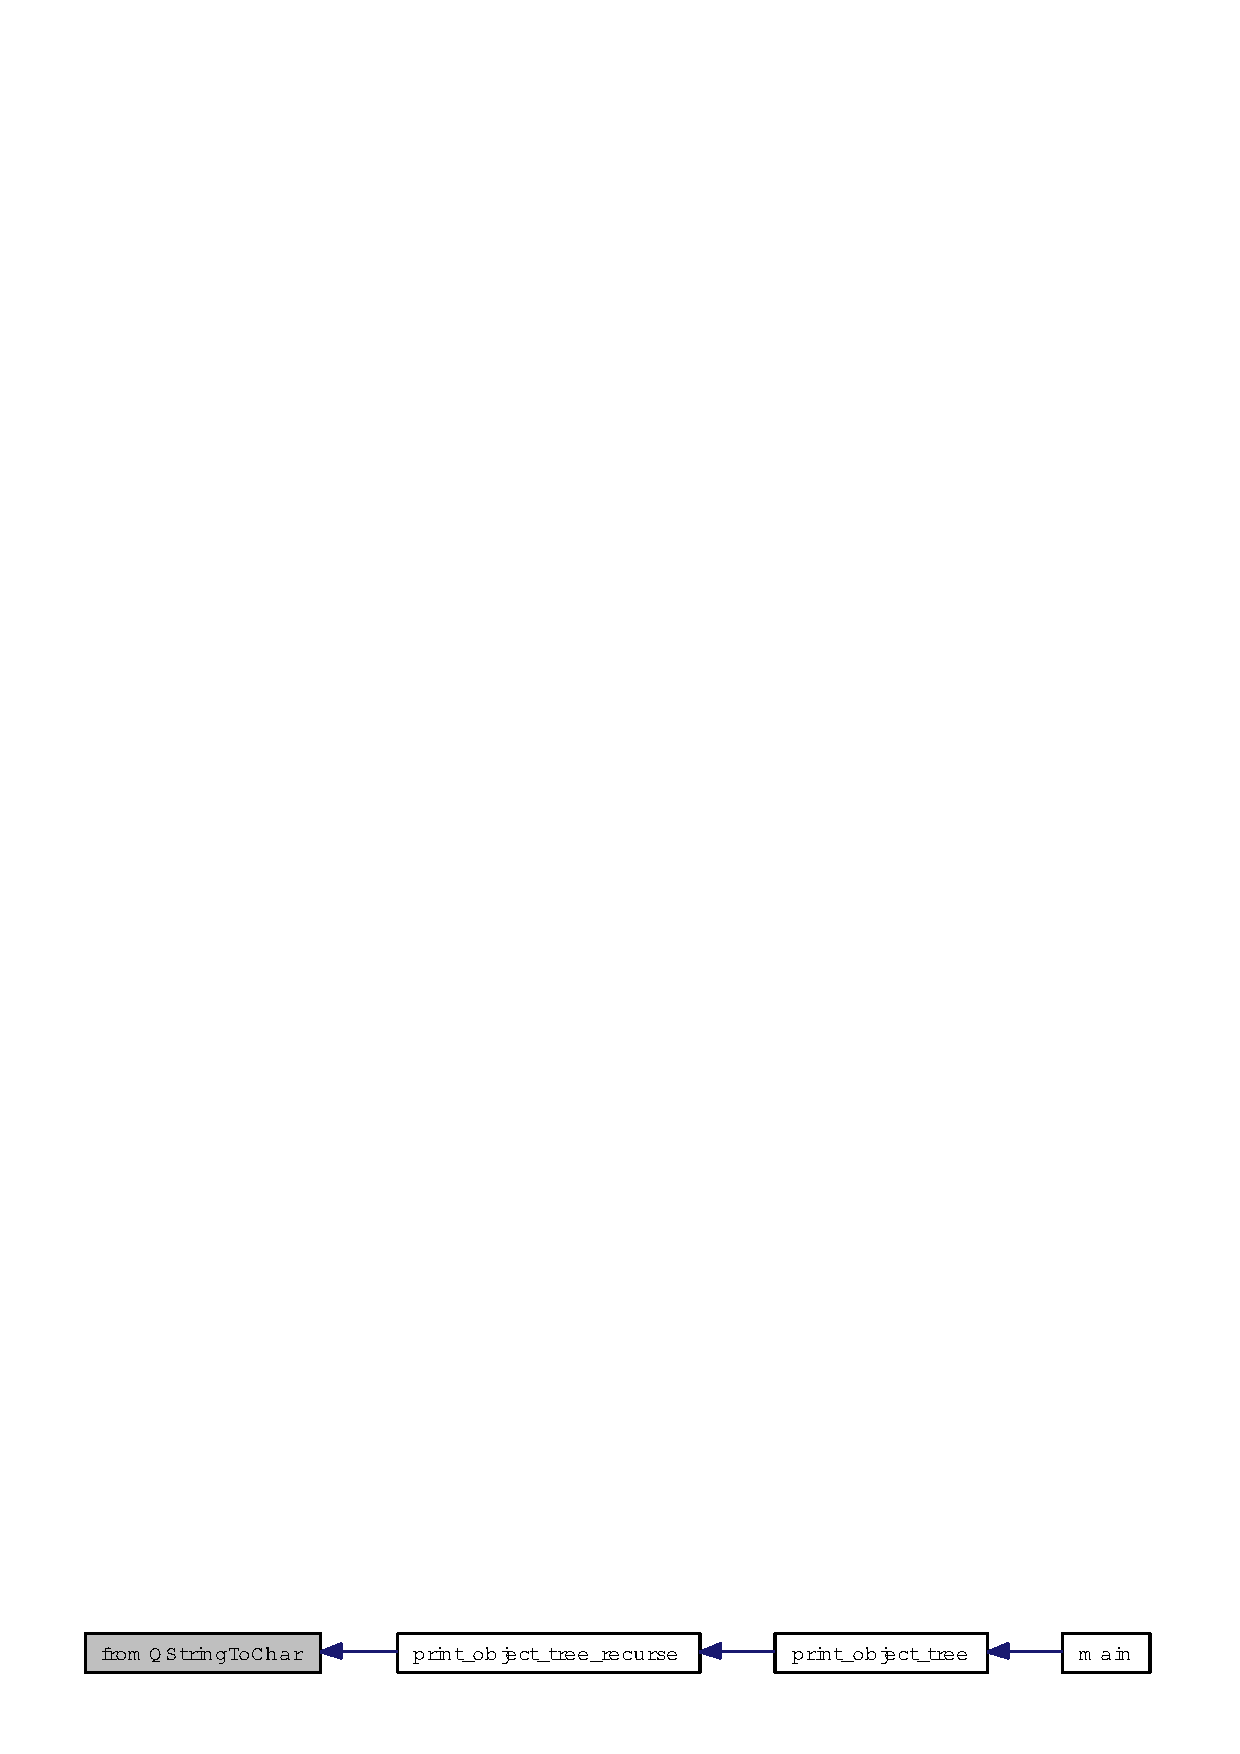
\includegraphics[width=278pt]{main_8cpp_0dda5f4014a4e3496449270026f6c149_icgraph}
\end{center}
\end{figure}
\index{main.cpp@{main.cpp}!imax@{imax}}
\index{imax@{imax}!main.cpp@{main.cpp}}
\subsubsection{\setlength{\rightskip}{0pt plus 5cm}int imax (int {\em x1}, int {\em x2})}\label{main_8cpp_99d8888037c7927cbe6362f80a2f6f8b}




Definition at line 229 of file main.cpp.\index{main.cpp@{main.cpp}!imin@{imin}}
\index{imin@{imin}!main.cpp@{main.cpp}}
\subsubsection{\setlength{\rightskip}{0pt plus 5cm}int imin (int {\em x1}, int {\em x2})}\label{main_8cpp_6c9ac00d126f1109a583b5264a07412a}




Definition at line 236 of file main.cpp.

Referenced by findscreen::setup\_\-toolsline(), and infofieldenter::setup\_\-ui().

Here is the caller graph for this function:\begin{figure}[H]
\begin{center}
\leavevmode
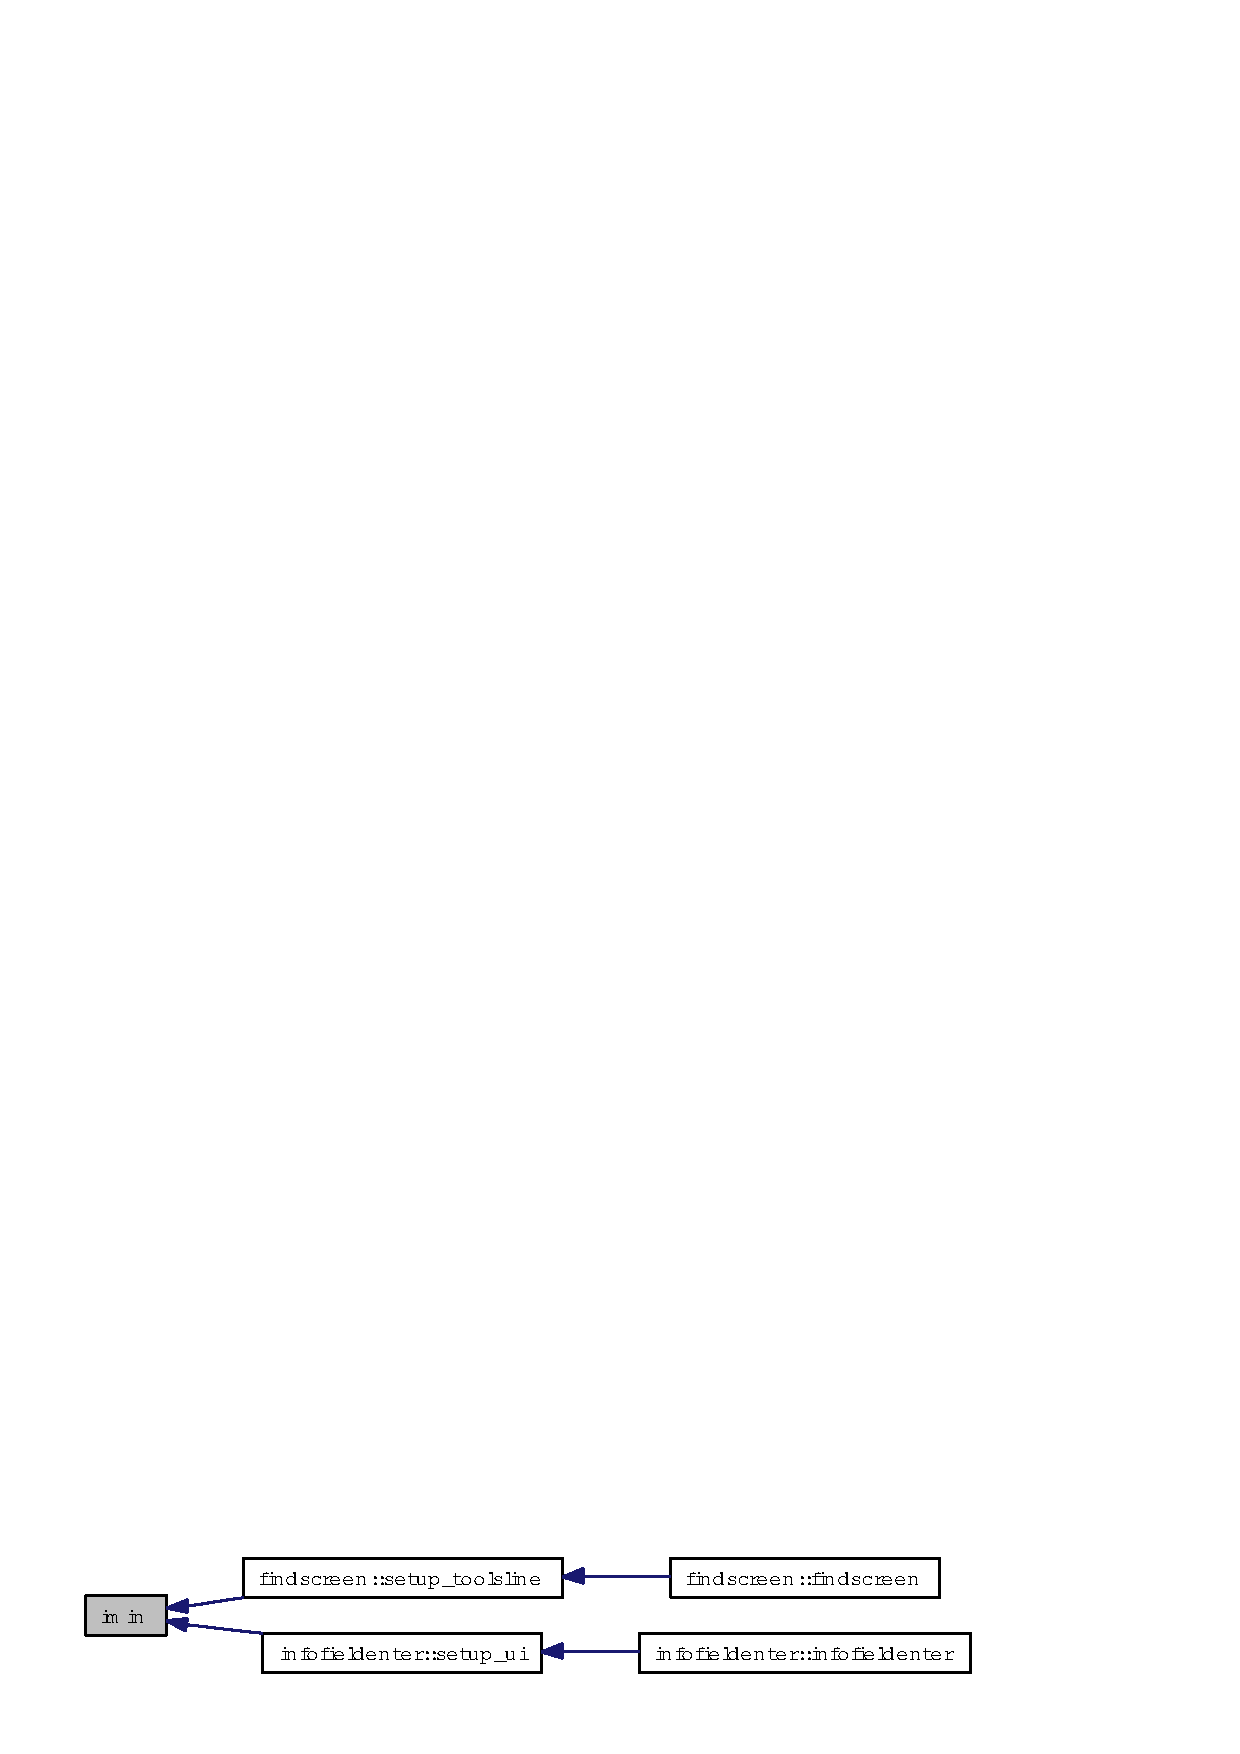
\includegraphics[width=235pt]{main_8cpp_6c9ac00d126f1109a583b5264a07412a_icgraph}
\end{center}
\end{figure}
\index{main.cpp@{main.cpp}!info_window@{info\_\-window}}
\index{info_window@{info\_\-window}!main.cpp@{main.cpp}}
\subsubsection{\setlength{\rightskip}{0pt plus 5cm}void info\_\-window (QString {\em i})}\label{main_8cpp_11a7110d2888630c2a28e17fcd3199fd}




Definition at line 50 of file main.cpp.

Referenced by editor::on\_\-showhtml\_\-clicked().\index{main.cpp@{main.cpp}!logprint@{logprint}}
\index{logprint@{logprint}!main.cpp@{main.cpp}}
\subsubsection{\setlength{\rightskip}{0pt plus 5cm}void logprint (char $\ast$ {\em lpsz\-Text},  {\em ...})}\label{main_8cpp_e8160c24b0b45e234c5ad305d0d31a3b}




Definition at line 12 of file main.cpp.\index{main.cpp@{main.cpp}!main@{main}}
\index{main@{main}!main.cpp@{main.cpp}}
\subsubsection{\setlength{\rightskip}{0pt plus 5cm}int main (int {\em argc}, char $\ast$$\ast$ {\em argv})}\label{main_8cpp_3c04138a5bfe5d72780bb7e82a18e627}




Definition at line 243 of file main.cpp.

References DPF, GAME\_\-RELEASE, GAME\_\-RELEASE\_\-VERSION, mainwindowpointer, print\_\-object\_\-tree(), mainwindow::restore\_\-findonbase\_\-visible(), mainwindow::restore\_\-geometry(), mainwindow::restore\_\-recordtable\_\-position(), and mainwindow::restore\_\-tree\_\-position().

Here is the call graph for this function:\begin{figure}[H]
\begin{center}
\leavevmode
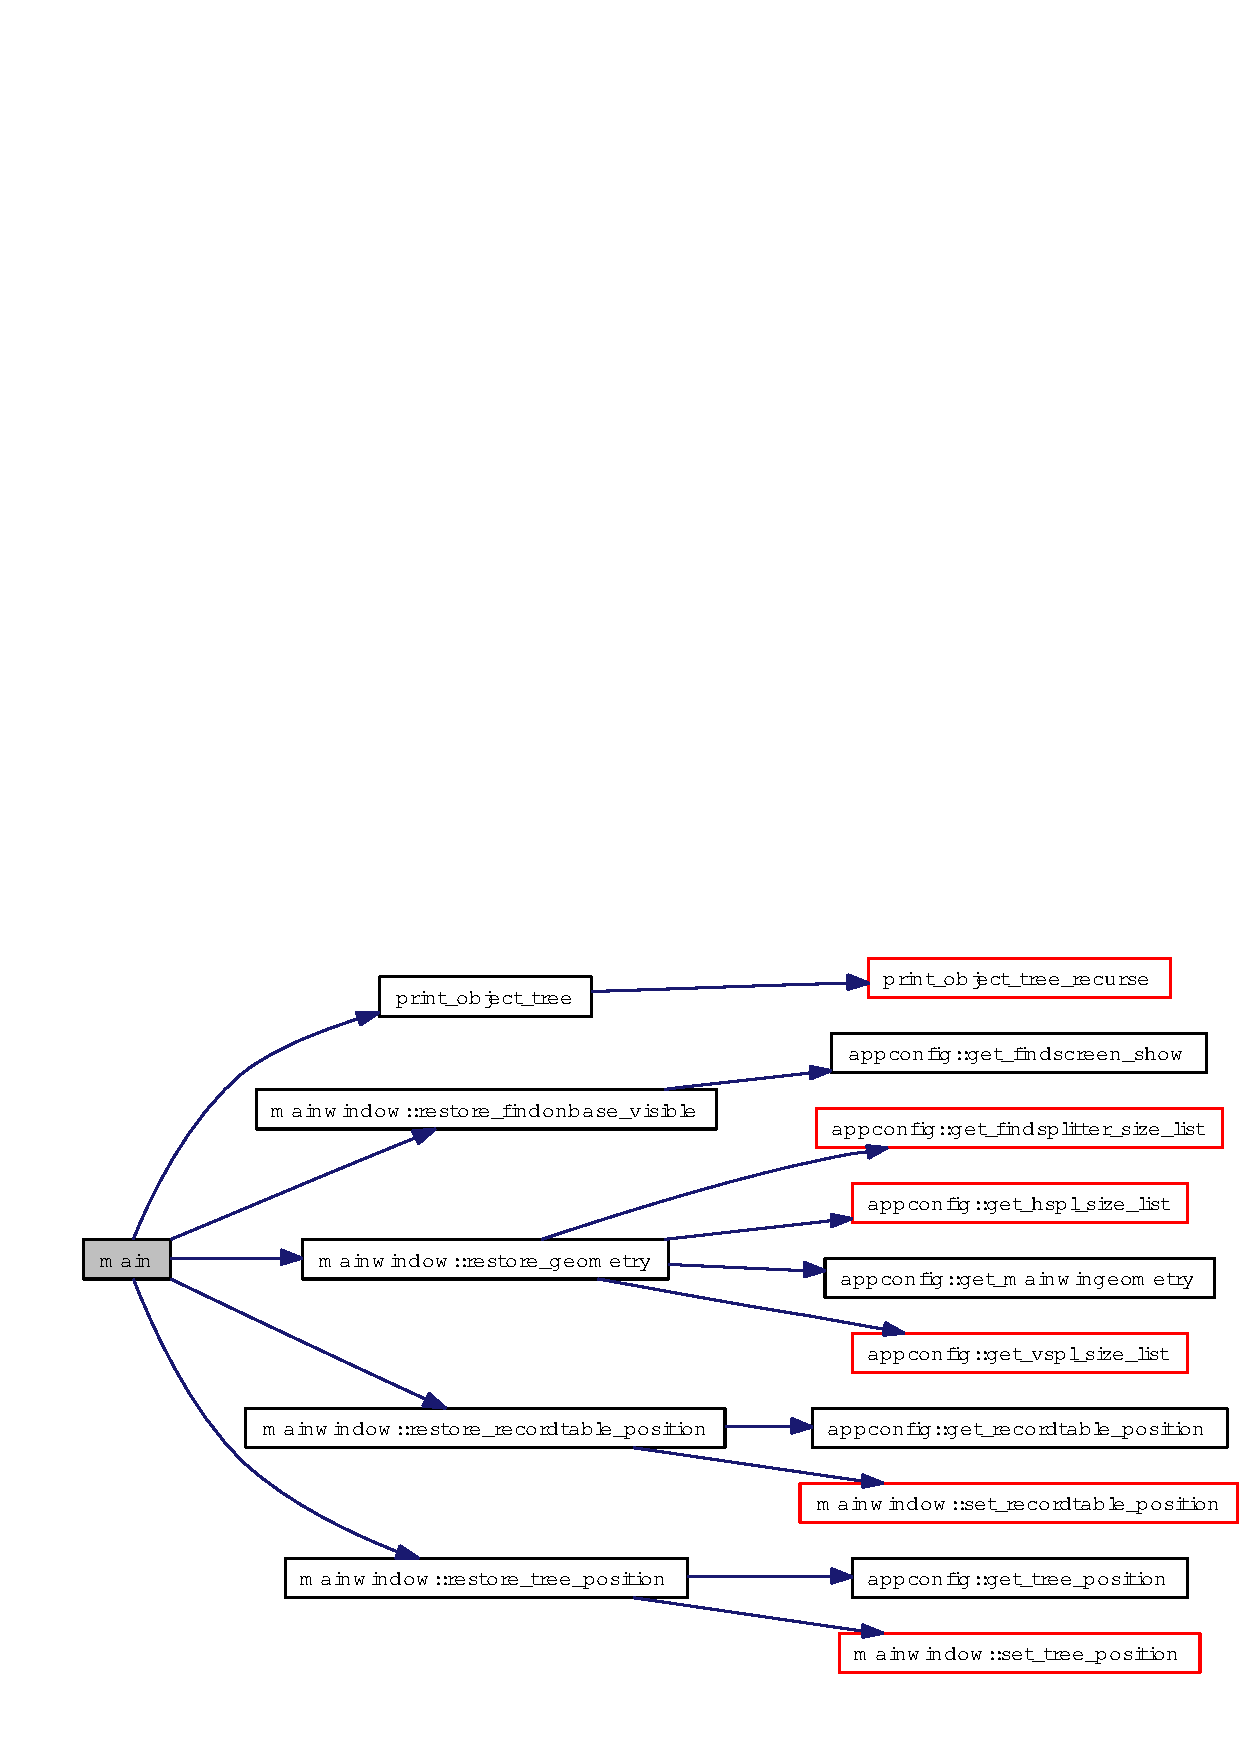
\includegraphics[width=299pt]{main_8cpp_3c04138a5bfe5d72780bb7e82a18e627_cgraph}
\end{center}
\end{figure}
\index{main.cpp@{main.cpp}!print_object_tree@{print\_\-object\_\-tree}}
\index{print_object_tree@{print\_\-object\_\-tree}!main.cpp@{main.cpp}}
\subsubsection{\setlength{\rightskip}{0pt plus 5cm}void print\_\-object\_\-tree (void)}\label{main_8cpp_8ff96661921f7c09201747e09d034951}




Definition at line 214 of file main.cpp.

References mainwindowpointer, and print\_\-object\_\-tree\_\-recurse().

Referenced by main().

Here is the call graph for this function:\begin{figure}[H]
\begin{center}
\leavevmode
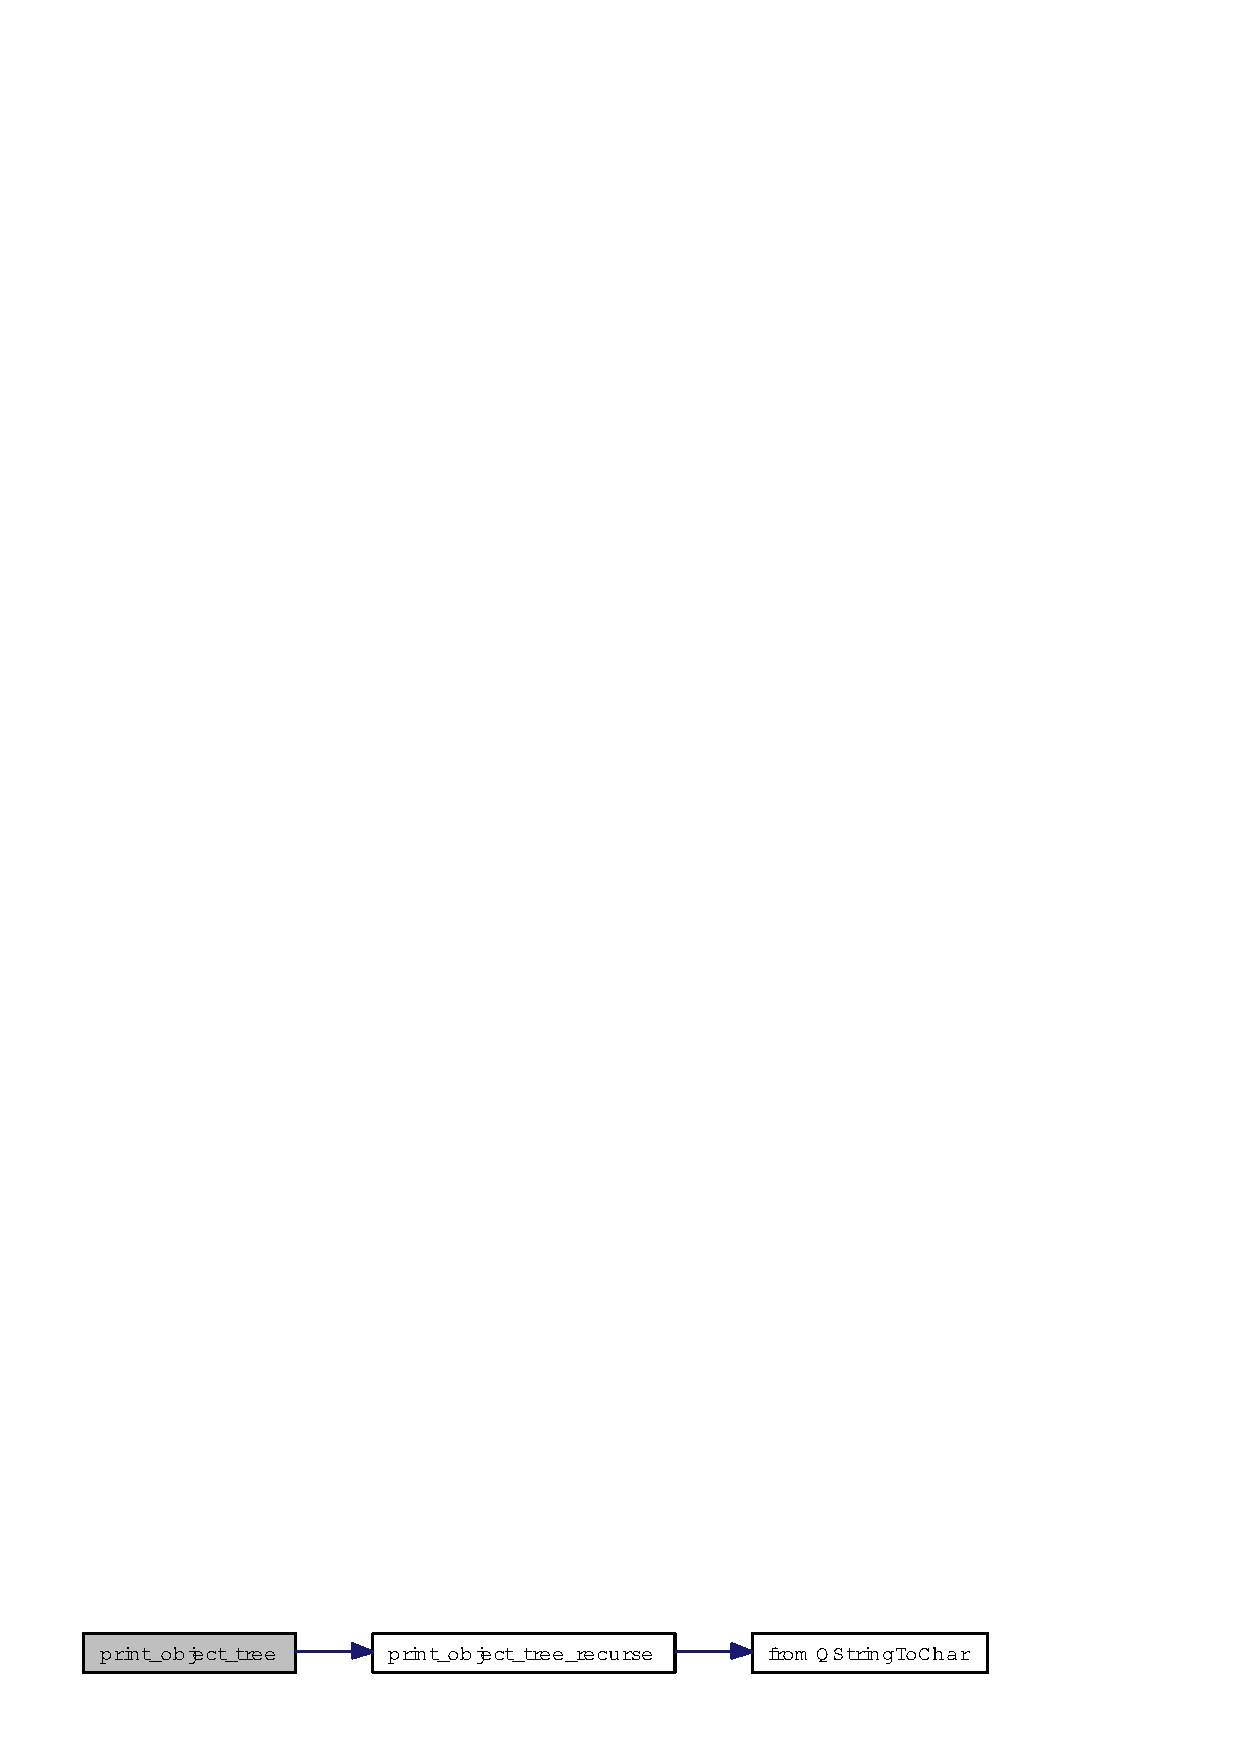
\includegraphics[width=239pt]{main_8cpp_8ff96661921f7c09201747e09d034951_cgraph}
\end{center}
\end{figure}


Here is the caller graph for this function:\begin{figure}[H]
\begin{center}
\leavevmode
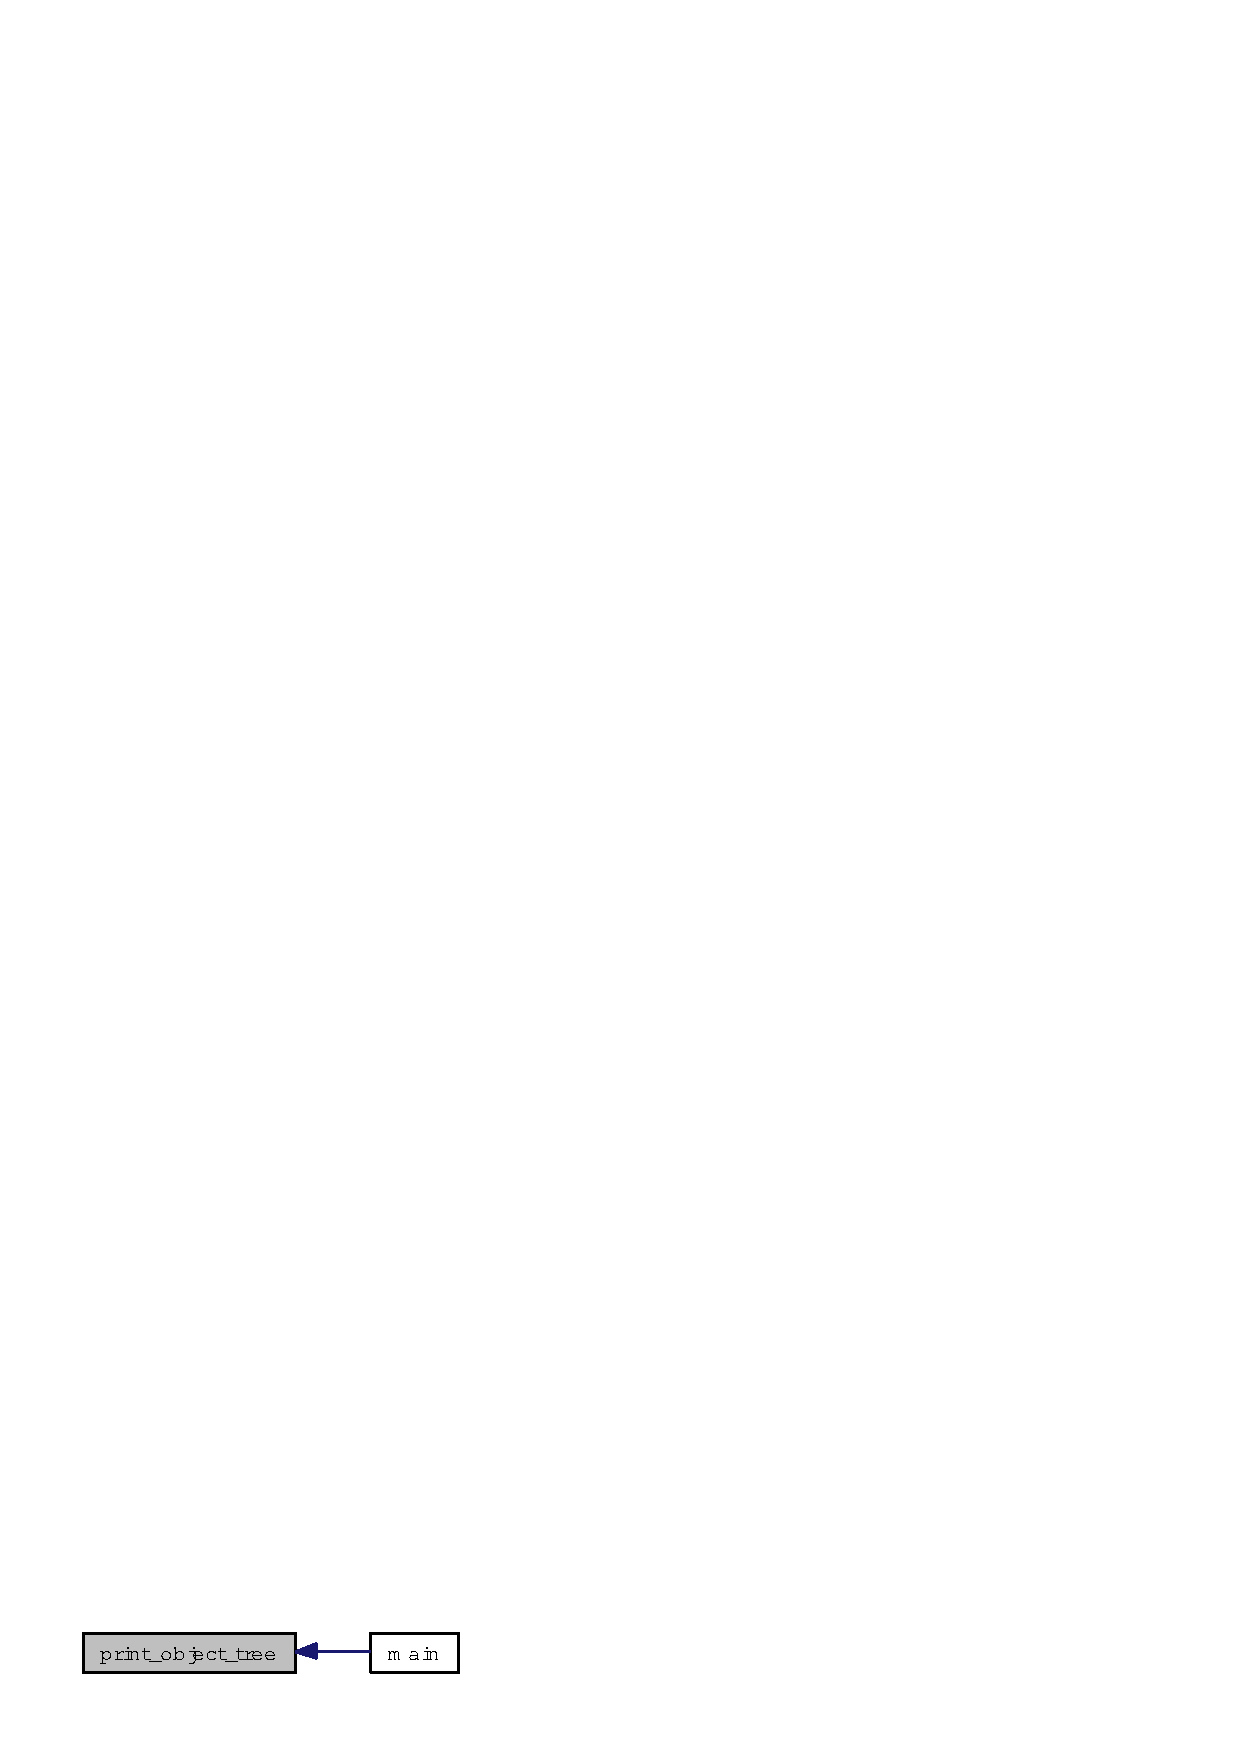
\includegraphics[width=112pt]{main_8cpp_8ff96661921f7c09201747e09d034951_icgraph}
\end{center}
\end{figure}
\index{main.cpp@{main.cpp}!print_object_tree_recurse@{print\_\-object\_\-tree\_\-recurse}}
\index{print_object_tree_recurse@{print\_\-object\_\-tree\_\-recurse}!main.cpp@{main.cpp}}
\subsubsection{\setlength{\rightskip}{0pt plus 5cm}void print\_\-object\_\-tree\_\-recurse (QObject $\ast$ {\em pobj})}\label{main_8cpp_571c71b2c6270a13685be239f6f91311}




Definition at line 185 of file main.cpp.

References from\-QString\-To\-Char().

Referenced by print\_\-object\_\-tree().

Here is the call graph for this function:\begin{figure}[H]
\begin{center}
\leavevmode
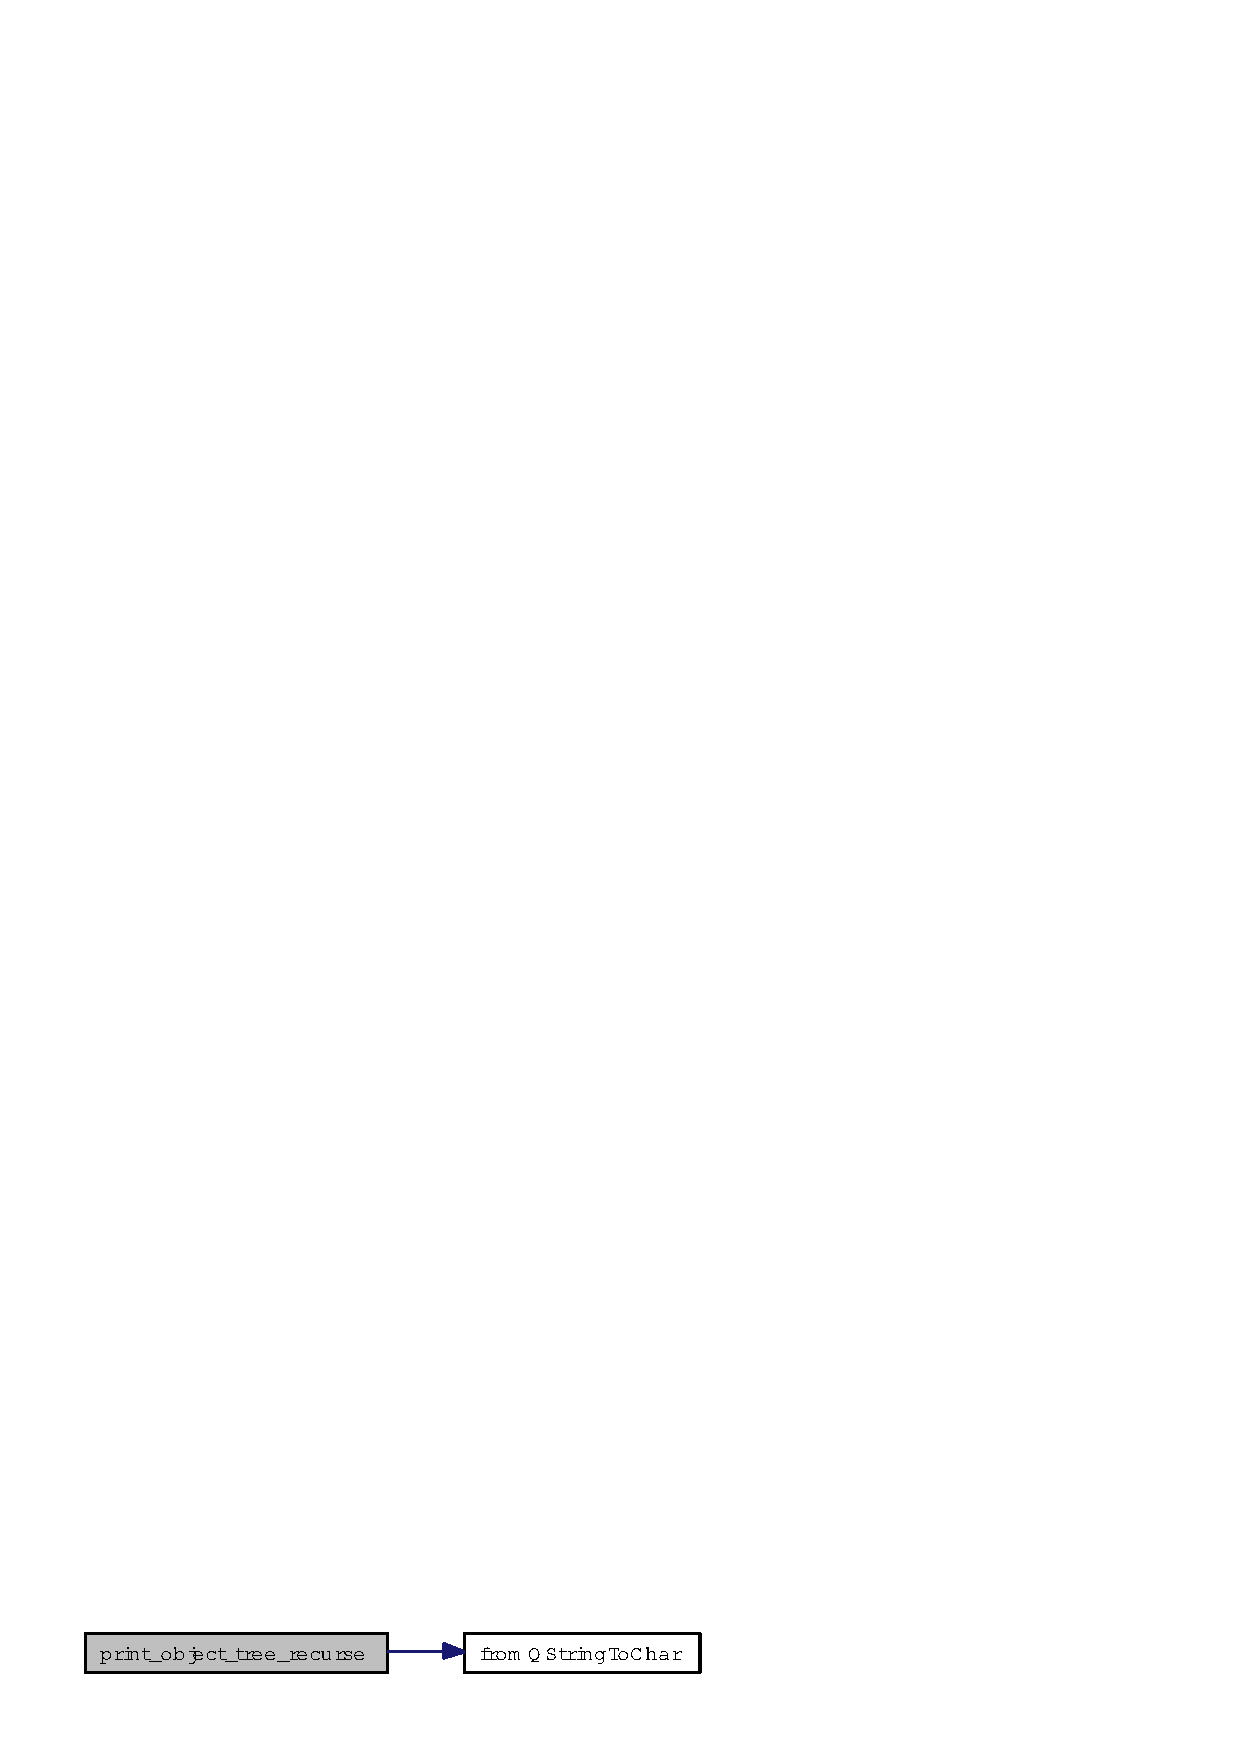
\includegraphics[width=170pt]{main_8cpp_571c71b2c6270a13685be239f6f91311_cgraph}
\end{center}
\end{figure}


Here is the caller graph for this function:\begin{figure}[H]
\begin{center}
\leavevmode
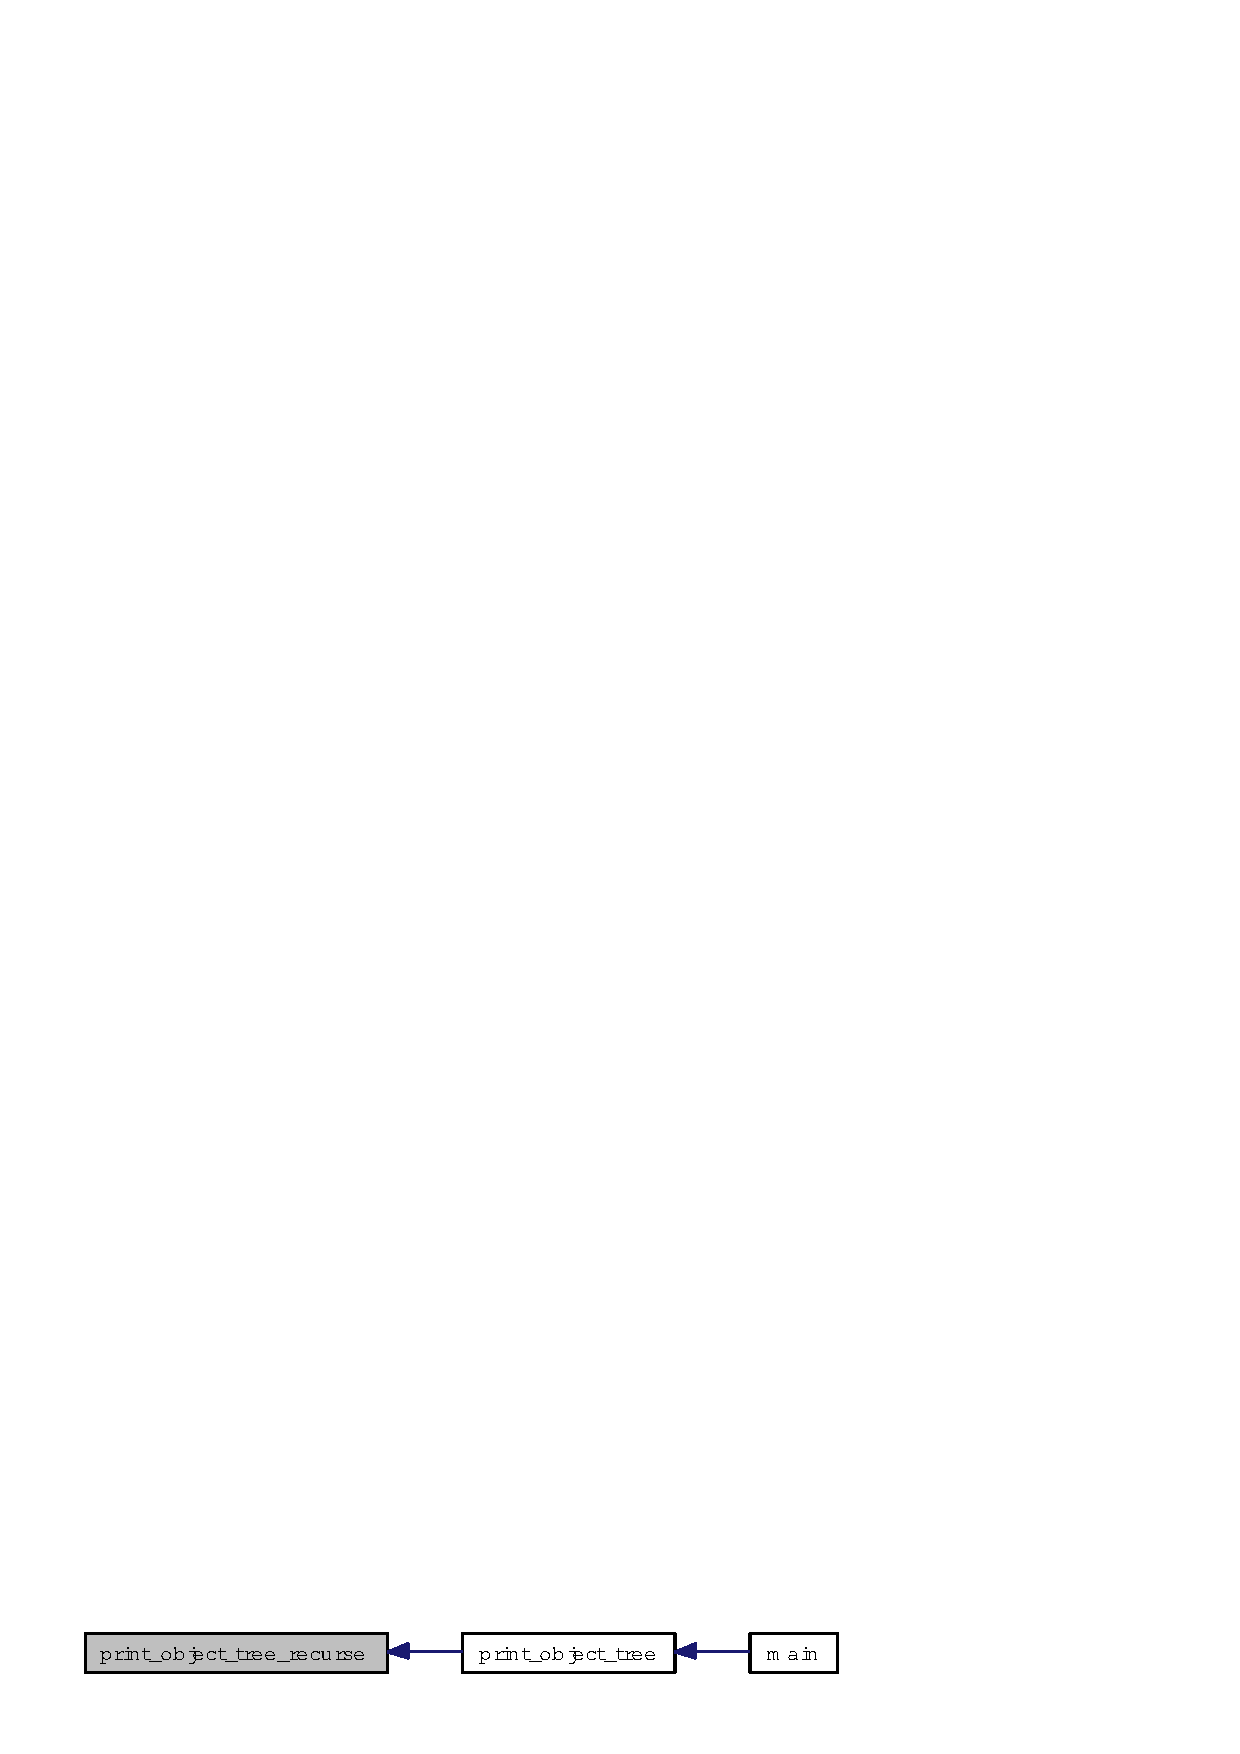
\includegraphics[width=203pt]{main_8cpp_571c71b2c6270a13685be239f6f91311_icgraph}
\end{center}
\end{figure}
\index{main.cpp@{main.cpp}!remove_dir@{remove\_\-dir}}
\index{remove_dir@{remove\_\-dir}!main.cpp@{main.cpp}}
\subsubsection{\setlength{\rightskip}{0pt plus 5cm}void remove\_\-dir (QString {\em namedirfrom})}\label{main_8cpp_6ac3f8d337a3e659a3c1cdfeef1cbaf0}




Definition at line 125 of file main.cpp.

References appconfig::get\_\-lastprefixnum\_\-as\_\-line(), appconfig::get\_\-trashdir(), appconfig::inc\_\-lastprefixnum(), and mytetraconfig.

Referenced by recordtabledata::delete\_\-record().

Here is the call graph for this function:\begin{figure}[H]
\begin{center}
\leavevmode
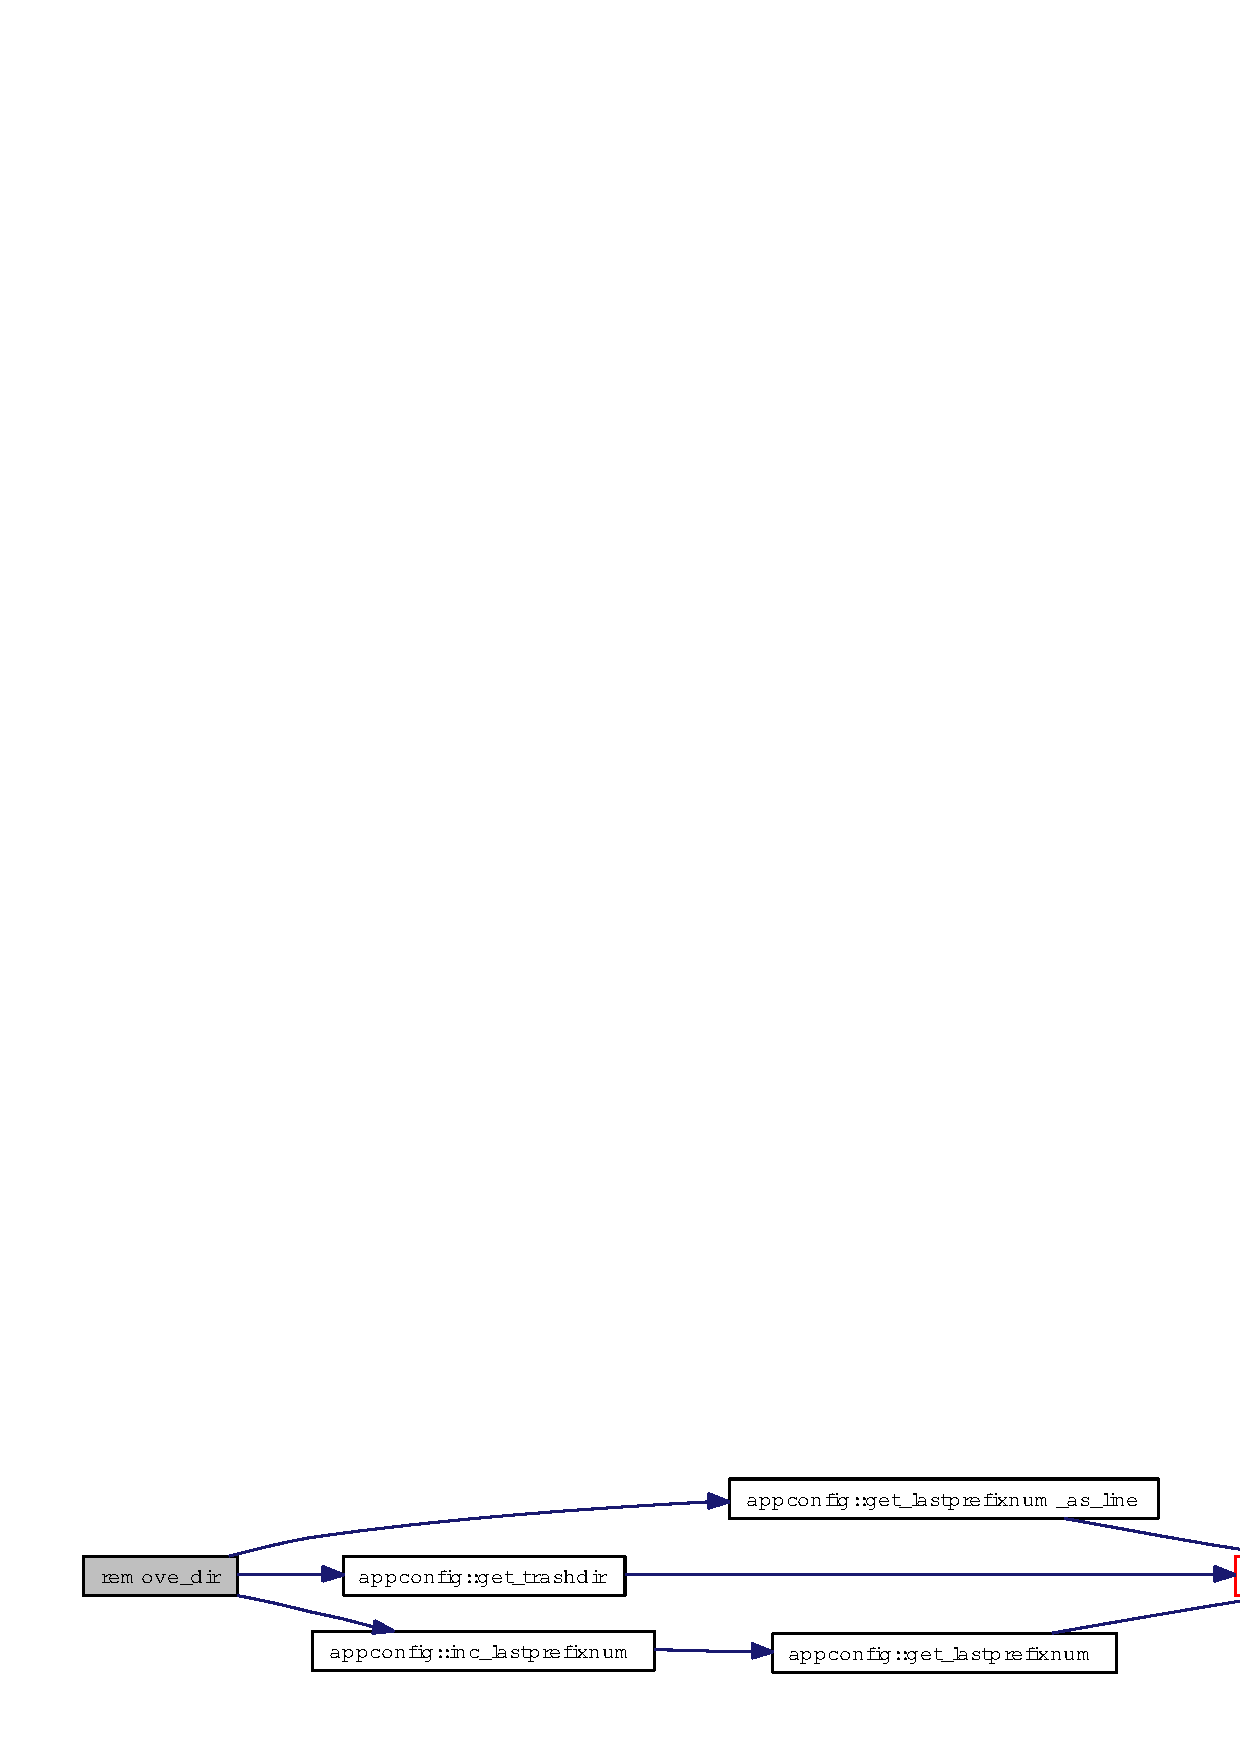
\includegraphics[width=373pt]{main_8cpp_6ac3f8d337a3e659a3c1cdfeef1cbaf0_cgraph}
\end{center}
\end{figure}


Here is the caller graph for this function:\begin{figure}[H]
\begin{center}
\leavevmode
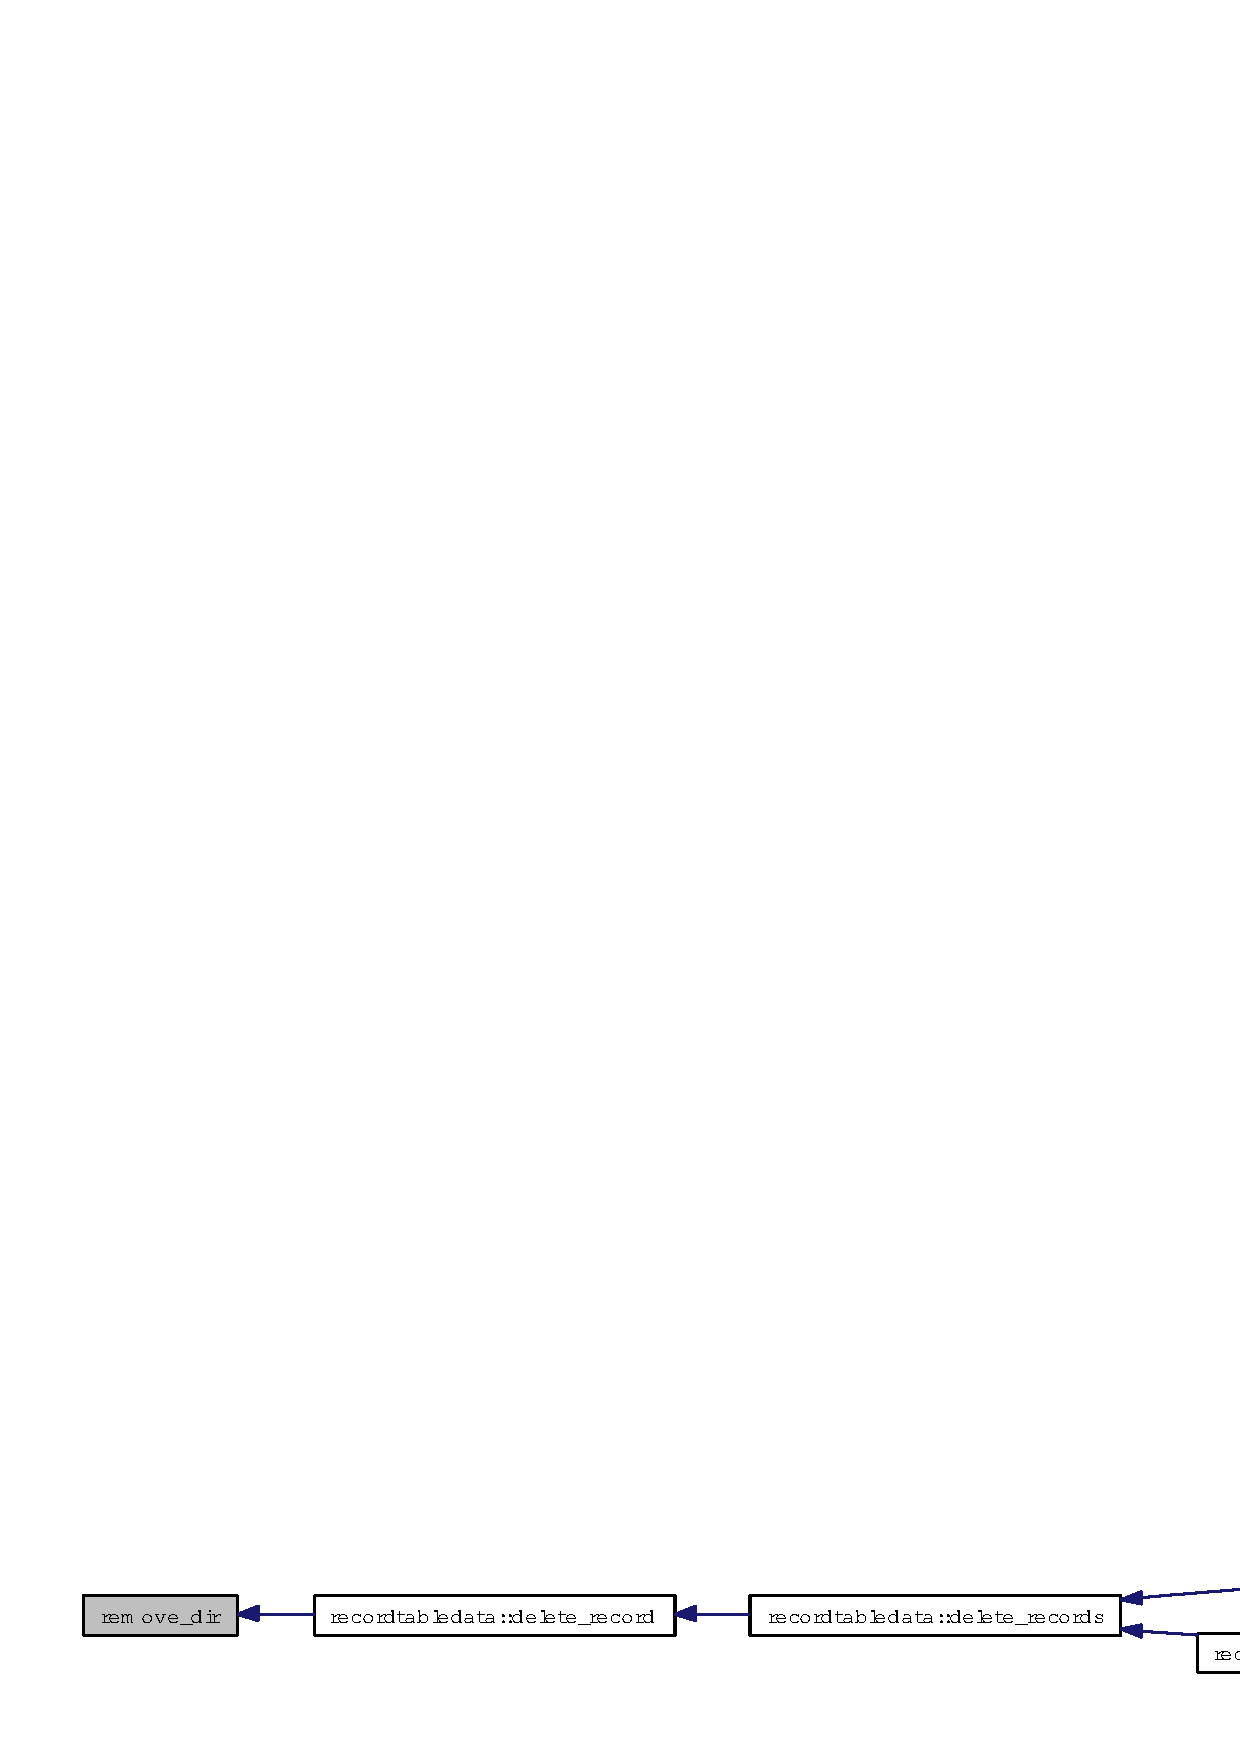
\includegraphics[width=384pt]{main_8cpp_6ac3f8d337a3e659a3c1cdfeef1cbaf0_icgraph}
\end{center}
\end{figure}
\index{main.cpp@{main.cpp}!xmlnode_to_string@{xmlnode\_\-to\_\-string}}
\index{xmlnode_to_string@{xmlnode\_\-to\_\-string}!main.cpp@{main.cpp}}
\subsubsection{\setlength{\rightskip}{0pt plus 5cm}QString xmlnode\_\-to\_\-string (QDom\-Node {\em xmldata})}\label{main_8cpp_dbcd54017c14dc5f88b7ff9e17a87706}




Definition at line 73 of file main.cpp.

\subsection{Variable Documentation}
\index{main.cpp@{main.cpp}!mainwindowpointer@{mainwindowpointer}}
\index{mainwindowpointer@{mainwindowpointer}!main.cpp@{main.cpp}}
\subsubsection{\setlength{\rightskip}{0pt plus 5cm}QObject$\ast$ {\bf mainwindowpointer}}\label{main_8cpp_8d16e0096a99e911957115d6d933ed13}




Definition at line 10 of file main.cpp.

Referenced by find\_\-object(), main(), and print\_\-object\_\-tree().\index{main.cpp@{main.cpp}!mytetraconfig@{mytetraconfig}}
\index{mytetraconfig@{mytetraconfig}!main.cpp@{main.cpp}}
\subsubsection{\setlength{\rightskip}{0pt plus 5cm}{\bf appconfig} {\bf mytetraconfig}}\label{main_8cpp_69bd0a7d678d494effdef51808501712}




Definition at line 7 of file main.cpp.